\documentclass{article}
\usepackage{graphicx}
\usepackage{amsmath,amsthm,amssymb}
\usepackage[font=small,labelfont=bf]{caption}
\usepackage{tikz}
\usetikzlibrary{calc, angles, quotes}
\usepackage{tkz-euclide}
\usepackage{float}
\usepackage[margin=1in]{geometry}
\usepackage{gensymb}
\usepackage{fancyhdr}
\pagestyle{fancy}
\fancyhead[R]{Enoch Yu}
\pagenumbering{gobble}
\usepackage{enumitem}
\newtheorem{theorem}{Theorem}[section]
\newtheorem{lemma}[theorem]{Lemma}
\newtheorem{sublemma}{Lemma}[section]
\newtheorem{proposition}{Proposition}
\newtheorem{corollary}{Corollary}[theorem]
\newenvironment{solution}{\begin{trivlist}\item[]{\bf Solution}}{\qed \end{trivlist}}

\title{Problem Set 4}
\author{Enoch Yu}
\date{May 2025}

\begin{document}

\section*{2023 AMC 12B Problem 16}
In Coinland, there are three types of coins, each worth $6, 10,$ and $15.$ What is the sum of the digits of the maximum amount of money that is impossible to have?
\\\\
$\textbf{(A) }8\qquad\textbf{(B) }10\qquad\textbf{(C) }7\qquad\textbf{(D) }11\qquad\textbf{(E) }9$
\\\\
\textbf{Solution I: During Test}
\\\\
\textbf{Key Word} Pattern Recognition
\\\\
The method is to utilize the fact that when a number could form with 6, 10 and 15, numbers formed by adding multiples of 6 to the initial number also could form. Number "6" was chosen to minimize the range of period of the pattern.
\\\\
Choose an arbitrary integer 20. \\
$20+6k$ is valid. \\
$21+6k$ is valid. \\
$22+6k$ is valid. \\
$23$ is not valid. \\
$24+6k$ is valid. \\
$25+6k$ is valid.
\\\\
It is likely that $23+6k$ produces the maximum amount of money that is impossible to have. 29 is impossible to have. However, from 35, moneys could form. Therefore, $2+9=\boxed{11}$.
\\\\
\noindent
\textbf{Solution II: Generalizing Method}
\\\\
\textbf{Key Word} Forming a Generalized Relationship
\\\\
Let $a,b\text{ and }c$ be the number of coins that worth 6, 10 and 13 respectively. If $6a+10b+15c=k$, then $6(a+1)+10(b-2)+15(c+1)=k+1$. The following represents the relationship between an arbitrary triple of $(a,b,c)$.
\[
\begin{array}{ccccccccccccc}
    (1,6,2) & \rightarrow & (2,4,3) & \rightarrow & (3,2,4) & \rightarrow & (4,0,5) & \leftarrow & (0,10,0) & \leftarrow & (1,8,1) & \leftarrow & (2,6,2) \\
    96 & & 97 & & 98 & & 99 & & 100 & & 101 & & 102
\end{array}
\]
By induction, it is evident that all natural numbers greater than or equal to 96 may form. Because a limit is given, same method used in Solution I may be utilized to obtain $\boxed{\textbf{(D) }11}$.

\newpage
\section*{2023 AMC 12B Problem 18}
Last academic year Yolanda and Zelda took different courses that did not necessarily administer the same number of quizzes during each of the two semesters. Yolanda's average on all the quizzes she took during the first semester was $3$ points higher than Zelda's average on all the quizzes she took during the first semester. Yolanda's average on all the quizzes she took during the second semester was $18$ points higher than her average for the first semester and was again $3$ points higher than Zelda's average on all the quizzes Zelda took during her second semester. Which one of the following statements cannot possibly be true?
\\\\
$\textbf{(A)}$ Yolanda's quiz average for the academic year was $22$ points higher than Zelda's. \\
$\textbf{(B)}$ Zelda's quiz average for the academic year was higher than Yolanda's. \\
$\textbf{(C)}$ Yolanda's quiz average for the academic year was $3$ points higher than Zelda's. \\
$\textbf{(D)}$ Zelda's quiz average for the academic year equaled Yolanda's. \\
$\textbf{(E)}$ If Zelda had scored $3$ points higher on each quiz she took, then she would have had the same average for the academic year as Yolanda.
\begin{solution}
\\\\
\textbf{Key Word} Property of Fraction
\\\\
Let
\begin{align*}
    \text{Yolanda's 1st Semester Average} &= \frac{a_1+\dots+a_n}{n} \\
    \text{Yolanda's 2nd Semester Average} &= \frac{a_1'+\dots+a_n'}{n'} \\
    \text{Zelda's 1st Semester Average} &= \frac{b_1+\dots+b_m}{m} \\
    \text{Zelda's 2nd Semester Average} &= \frac{b_1'+\dots+b_m'}{m'}.
\end{align*}
According to the problem, $\frac{a_1+\dots+a_n}{n}+18=\frac{a_1'+\dots+a_n'}{n'}$. Moreover, $\frac{a_1+\dots+a_n}{n}=\frac{b_1+\dots+b_m}{m}+3$ and $\frac{a_1'+\dots+a_n'}{n'}=\frac{b_1'+\dots+b_m'}{m'}+3$ are true. In another words,
\[
\frac{a_1+\dots+a_n}{n}=\frac{a_1'+\dots+a_n'-18n'}{n'}=\frac{b_1+\dots+b_m+3m}{m}= \frac{b_1'+\dots+b_m'-15m'}{m'}.
\]
The relationship leads to
\[
\frac{a_1+\dots+a_n+a_1'+\dots+a_n'-18n'}{n+n'}=\frac{b_1+\dots+b_m+b_1'+\dots+b_m'+3m-15m'}{m+m'}, \text{or}
\]
\[
\frac{a_1+\dots+a_n+a_1'+\dots+a_n'}{n+n'}-\frac{18n'}{n'+n}-\frac{3m}{m+m'}+\frac{15m'}{m+m'}=\frac{b_1+\dots+b_m+b_1'+\dots+b_m'}{m+m'}.
\]
For choice $(A)$ to be true, $-\frac{18n'}{n'+n}-\frac{3m}{m+m'}+\frac{15m'}{m+m'}$ must be $-22$. \\
Let $n'=kn$ and $m'=k'm$.
\[
-\frac{18n'}{n'+n}-\frac{3m}{m+m'}+\frac{15m'}{m+m'}=-\frac{18kn}{n(k+1)}-\frac{3m}{m(k'+1)}+\frac{15k'm}{m(k'+1)}=-\frac{18kn}{n(k+1)}+\frac{3m(5k'-1)}{m(k'+1)}
\]
$n,n',m,m',k\text{ and }k'$ must be non-zero integer to satisfy the condition in the question. While the equation above is a multiple of three, 22 is not. Therefore, choice $\boxed{(A) \text{ cannot be true.}}$
\end{solution}

\newpage
\section*{2023 AMC 12B Problem 20}
Cyrus the frog jumps $2$ units in a direction, then $2$ more in another direction. What is the probability that he lands less than $1$ unit away from his starting position?
\\\\
$\textbf{(A)}~\frac{1}{6}\qquad\textbf{(B)}~\frac{1}{5}\qquad\textbf{(C)}~\frac{\sqrt{3}}{8}\qquad\textbf{(D)}~\frac{\arctan \frac{1}{2}}{\pi}\qquad\textbf{(E)}~\frac{2\arcsin \frac{1}{4}}{\pi}$
\begin{solution}
\\\\
\textbf{Key Word} Law of Cosines, Inverse Trigonometric Identities
\\\\
WLOG, the probability that Cyrus lands less than 1 unit away from the starting position is 
\[
\frac{\text{Length of Red Curve}}{\text{Length of Red Curve + Length of Blue Curve}}.
\]
\begin{center}
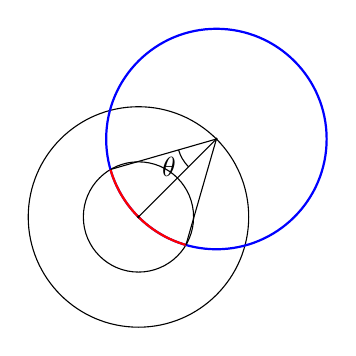
\begin{tikzpicture}[scale=0.7]
    \coordinate (O) at (0,0);
    \coordinate (A) at (1.41421356237,1.41421356237);
    \coordinate (B) at (-0.50788, 0.86143);
    \coordinate (C) at (0.86143, -0.50788);

    \draw (O) circle (1);
    \draw (O) circle (2);
    \draw[color=blue, thick] (A) circle (2);

    \pgfmathsetmacro{\angleB}{atan2(0.86143 - 1.41421356237, -0.50788 - 1.41421356237)}
    \pgfmathsetmacro{\angleC}{atan2(-0.50788 - 1.41421356237, 0.86143 - 1.41421356237)}

    \draw[red, thick] (A) ++(\angleB:2) arc[start angle=\angleB, end angle=\angleC, radius=2];

    \draw (A) -- (B);
    \draw (A) -- (C);
    \draw (A) -- (O);

    \node at (O)[circle,fill,inner sep=0.4pt]{};
    \node at (A)[circle,fill,inner sep=0.4pt]{};

    \draw pic[draw=black, radius=0.5cm, "$\theta$", angle eccentricity=1.4] {angle=B--A--O};
\end{tikzpicture}
\end{center}
The length of blue curve and red curve is the circumference of a circle with radius of 2, or $4\pi$. The length of the red curve may be found by computing the value of $\theta$, where $\theta$ is in radians for convenience. Using Law of Cosines, $\cos\theta=\frac{2^2+2^2-1^2}{2\cdot2\cdot2}=\frac{7}{8}$. Using a right triangle with lengths $7,8\text{ and }\sqrt{15}$, it is evident that $\sin\theta=\frac{\sqrt{15}}{8}$.
\begin{align*}
    \text{Probability}&=\frac{4\pi\cdot\frac{2\theta}{2\pi}}{4\pi} \\
    &=\frac{\theta}{\pi}\\
\end{align*}
Assume $(E)$ is the correct answer. If $\arcsin{\frac{\sqrt{15}}{8}}=2\arcsin{\frac{1}{4}}$ is true, choice $(E)$ is the answer.
\begin{align*}
    \arcsin{\frac{\sqrt{15}}{8}}&=2\arcsin{\frac{1}{4}} \\
    \sin\left(\arcsin{\frac{\sqrt{15}}{8}}\right)&=\sin\left(2\arcsin{\frac{1}{4}}\right) \\
    \frac{\sqrt{15}}{8}&=2\cdot\sin\left(\arcsin{\frac{1}{4}}\right)\cdot\cos\left(\arcsin{\frac{1}{4}}\right) \\
    \frac{\sqrt{15}}{8}&=2\cdot\frac{1}{4}\cdot\sqrt{1-\left(\frac{1}{4}\right)^2} \\
    \frac{\sqrt{15}}{8}&=\frac{\sqrt{15}}{8} \\
\end{align*}
Therefore, the probability that Cyrus lands less than 1 unit away from his starting position is $\boxed{\textbf{(E)}~\frac{2\arcsin \frac{1}{4}}{\pi}}$.
\end{solution}

\end{document}
